\section{Einleitung}
In diesem Versuch wird das Verhalten von polarisiertem Licht untersucht.
\subsection{Polarisation durch Reflexion}
Es wird von linear polarisiertem Licht gesprochen, wenn der E-Feldvektor in nur einer Raumrichtung schwingt und von zirkular polarisiertem Licht wenn der E-Feldvektor eine Schraubenlinie beschreibt. Es wird elliptisch polarisiert genannt, wenn der E-Feldvektor eine Ellipse beschreibt.
Trifft Licht auf eine Glasfläche mit Brechungsindex $ n $ wird der Strahl teilweise reflektiert und teilweise gebrochen. Der Anteil des reflektierten Strahles hängt vom Einfallswinkel $ \alpha $ und von der Polarisation des Lichts ab.
Dabei hat senkrecht zur Einfallsebene Polarisiertes Licht (s-polarisiert) ein größeres Reflexionsvermögen als parallel zur Einfallsebene Polarisiertes Licht (p-polarisiert).
Dabei gibt es für p-polarisiertes Licht einen Einfallswinkel $ \alpha_{B} $ bei welchem kein Licht reflektiert wird, es gilt
\begin{equation}
\tan \alpha_{B} = n	\label{eq:brew}
\end{equation}
somit ist das reflektierte Licht vollständig linear s-polarisiert.
\subsection{Doppelbrechung in Kalkspat}
Beim Durchgang von unpolarisierten Licht durch den Kalkspatkristall, wird dieser in zwei Teilstrahlen aufgeteilt.
Ein Strahl verhält sich nach dem Snelliusschen Brechungsgesetz und wird daher auch ordentlicher Strahl genannt, für diesen gilt der Brechungindex $ n_{O} $. Der andere Teilstrahl wird außerordentlicher Strahl genannt, für diesen gilt der Brechungsindex $ n_{a} $. Die beiden Teilstrahlen sind orthogonal zueinander polarisiert. Der ordentliche Strahl ist s-polarisiert und der außerordentliche Strahl ist p-polarisiert.
\subsection{Polarisation durch selektive Absorption}
Polarisator und Analysator sind zwei einfache Polarisationsfilter. Fällt unpolarisiertes
Licht auf so einen Filter, wird dieser Polarisator genannt. Mit einem
zweiten Filter, dem Analysator, kann man nun untersuchen, ob z.B. die Polarisationsebene
sich gedreht hat. Die Komponente $\vec E = \vec E_0 \cos\varphi$ wird durchgelassen und die Komponente $\vec E' = \vec E_0 \cos\varphi$ wird absorbiert, wenn $\varphi$ der Winkel zwischen den Filtern ist. Da der gemessene Kurzschlussstrom eines Photoelements proportional der Lichtintensität I ist, folgt das \textit{Gesetz von Malus}
\begin{equation}
I = I_0 \cos^2\varphi \label{eq:malus}
\end{equation}
\subsection{$ \lambda/2 $-Platte}
Häufig ist es von Vorteil die Schwingungsebene von linear polarisiertem Licht um einen Winkel $ \bigtriangleup\alpha $ zu drehen. Mit einer $ \lambda/2-Platte $ ist dies möglich. Wenn der $ \vec{E}-Vektor $ den Winkel $ \varphi $ gegen die optische Achse hat, so kann dieser in zwei Komponenten aufspalte. Diese sind einmal der parallele Anteil $ E_{\|} = E\cos \varphi $ und der senkrechte Anteil $ E_{\bot}=E\sin \varphi $ . Treffen die beiden Komponente in die Platte ein sind sie in Phase. Die Komponenten haben unterschiedliche Laufzeiten, so entsteht zwischen ihnen eine Phasendifferenz $\bigtriangleup\varphi $. Es gilt, 
\begin{equation}
\bigtriangleup\varphi=\frac{2\pi}{\lambda}d(n_{2}-n_{1})
\end{equation}
$d$ ist die Strecke die durchlaufen wird. Bei der $ \lambda/2 - Platte $ gilt, $ d(n_{2}-n_{1})=\lambda/2 $, also $ \bigtriangleup\varphi=\pi $. Dabei hat sich der $ \vec{E}-Vektor $ um den Winkel $\bigtriangleup=2\varphi $ Durch das drehen der $ \lambda/2-Platte $ lässt sich jeder Winkel und somit jede gewünschte Drehung herbeiführen.
\subsection{Optische Aktivität}
Diese Medien, z.B. eine Zuckerlösung, haben die Eigenschaft die Polarisationsebene linear polarisierten Lichts zu drehen. Generell fehlen solchen Substanzen bestimmte Symmetrieeigenschaften - Kristalle ohne Symmetriezentrum, Moleküle ohne Symmetriezentrum und Ebene, in allen Zustandsformen. Die Kristalle oder Moleküle sind in einer Lösung zwar statistisch verteilt, zeigen diese Eigenschaften aber trotzdem: Die Lichtwelle wird von der Substanz in eine Richtung gedreht, aber nicht in die andere Richtung zurück, da die Substanz "'auf der Rückseite`` nicht die selben Eigenschaften besitzt, da es nicht symmetrisch ist. Durchdringt eine Lichtwelle nun so eine Substanz, die in Lösung ist, so hängt der Drehwinkel $\alpha$ von der Konzentration $c$ und der durchdrungenen Länge $l$ proportional ab:
\begin{equation}
\alpha = \alpha_{s}\cdot c\cdot l \label{eq:opt_akt}
\end{equation}
$\alpha_{s}$ ist der Proportionalitätsfaktor und heißt spezifische Drehung.
\newpage
\section{Auswertung}
\subsection{Überprüfung des Gesetz von Malus}
Das Gesetz von Malus gibt den Zusammenhang \eqref{eq:malus} zwischen transmittierter Lichtintensität und Winkel des Polarisators an.\\
Um den Zusammenhang nachzuweisen wird die Intensität von Licht, dass durch zwei Polarisatoren
gemessen. Da die Spannung am Photoelement proportional zur Lichtintensität ist, wird mit dieser Stellvertretend gearbeitet. Durch den ersten Polarisator wird die Polarisationsebene festgelegt. Diese wird im Verlauf der Messung beibehalten. Der zweite Polarisator wird zunächst so eingestellt, dass die Menge des transmittierten Lichts minimal wird. Daraufhin wird in \SI{10}{\degree}-Schritten die Spannung am Photoelement gemessen über einen Winkelbereich von insgesamt \SI{180}{\degree}.\\
Die von uns erhaltenen Messwerte sind im Laborbuch zu finden. Zur Auswertung haben wir diese Noch um eine Spannung von \SI{2+-1}{mV} bereinigt, die ohne einfallendes Licht gemessen wird.
Die um den systematischen Fehler bereinigten Messwerte haben wir mit Hilfe von \textit{Gnuplot} nach dem \textit{Least-Square-Fit} Verfahren gegen eine Funktion $ I(\alpha)  = I_0 \cos^2(\alpha-\alpha_0)$ gefittet. Abweichend von der Theorie taucht bei uns noch ein weiterer Summand im Argument des Kosinus auf, da wir die Winkel nicht in Bezug zur Polarisationsebene gemessen haben. Die bereinigten Werte und der dazugehörige Fit sind in Abbildung \ref{fig:malus} zu sehen.
\begin{figure}[H]
\centering
\def\h{10cm}
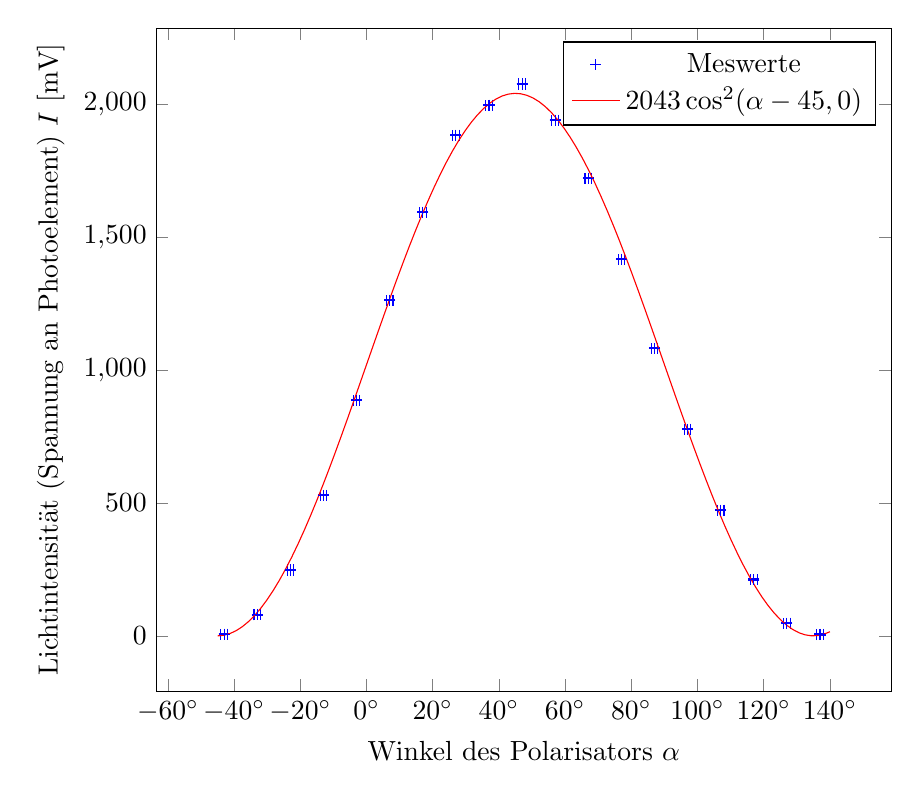
\begin{tikzpicture}
\begin{axis}[xticklabel=$\pgfmathprintnumber{\tick}^\circ$, width=.9\linewidth, height=\h,
	ylabel = {Lichtintensität (Spannung an Photoelement) $ I $ [\si{mV}]},
	xlabel = {Winkel des Polarisators $ \alpha $}]
	\addplot+ [only marks, mark=+, 
		error bars/.cd, x dir = both, x fixed=1,
		y dir = both, y fixed = 2] 
	table[x=x,y=y, x error=xerr, y error=yerr] {
x	xerr	y	yerr
137	1	5	2
127	1	48	2
117	1	212	2
107	1	473	2
97	1	778	2
87	1	1083	2
77	1	1418	2
67	1	1723	2
57	1	1942	2
47	1	2078	2
37	1	1998	2
27	1	1885	2
17	1	1595	2
7	1	1264	2
-3	1	887	2
-13	1	529	2
-23	1	248	2
-33	1	79	2
-43	1	6	2
	};
	\addplot+[domain= -45:140, no marks, samples=100] {2043*(cos(x - 44.9940891727))^2};
\legend{Meswerte, $ 2043\cos^2(\alpha-\SI{45,0}{\degree}) $}
\end{axis}

\end{tikzpicture}
\caption{Malus-Kurve}
\label{fig:malus}
\end{figure}
\subsection{$ \lambda/2 $-Platte}
Nun sollen die Eigenschaften der $ \lambda /2 -Platte $ untersucht werden.
Zuerst sollte geprüft werden, ob die $ \lambda /2 -Platte $ bei $ \SI{45}{\degree} $ die Polarisationsebene tatsächlich um $ \SI{90}{\degree} $ dreht. Um das zu untersuchen, wurden die Polarisationsfilter zunächst so eingestellt, dass der Relativwinkel $ 0^\circ $ beträgt. Ohne $ \lambda /2 -Platte $ wäre die gemessene Intensität maximal. Bringt man die $ \lambda /2 -Platte $ hinter den ersten Polarisationsfilter so wird eine minimale Intensität gemessen. Werden nun die Polarisationsfilter so eingestellt, dass der Relativwinkel $ 90^\circ $ beträgt, so wird ohne $ \lambda /2 -Platte $ ein Minimum gemessen. Mit $ \lambda /2 -Platte $ wird hier ein Maximum gemessen.
Wird die $ \lambda /2 -Platte $ auf $ 30^\circ $ eingestellt so ist ein Minimum bei einem Relativwinkel von $ 30^\circ $ messbar und ein Maximum bei einem Relativwinkel von $ 120^\circ $.

\subsection{Reflexion von p- und s-polarisierten Licht}
In diesem Versuch wird die Reflexion von Licht an einer Glasplatte in Abhängigkeit der Polarisationsrichtung untersucht. Dazu wird die Lichtintensität des an einer Glasscheibe reflektierten Lichts in Abhängigkeit vom Winkel gemessen. Als Lichtintensität wird die am Photosensor gemessene Spannung angenommen, da diese proportional zur einfallenden Lichtmenge ist. Dies führt man sowohl mit Licht durch, dass senkrecht zur Brechungsebene polarisiert einfällt, als auch mit Licht, das parallel zur Brechungsebene polarisiert einfällt. Zudem misst man die Lichtintensität, wenn das Licht direkt, also ohne von der Glasplatte beeinflusst zu werden, in den Photosensor fällt. Daraus lässt sich dann das Verhältnis von reflektierten zu einfallenden Licht bestimmen.\\
Bei der Messung ist uns aufgefallen, dass nicht nur ein, sondern zwei reflektierte Lichtpunkte zu sehen sind. Auf eine mögliche Begründung gehen wir in der Diskussion ein. Während der Durchführung kam dadurch erschwerend hinzu, dass man den Sensor immer wieder passend auf einen Lichtpunkt ausrichten muss. Um möglichst vergleichbare Messungen durchzuführen haben wir den Sensor jeweils so ausgerichtet, dass die gemessene Spannung maximal wird.\\
Von unsere Messwerten, die im Laborbuch zu finden sind, haben wir zunächst den Spannungswert den wir an der Photodiode ohne einfallendes Licht messen abgezogen. Damit minimieren wir den systematischen Fehler. Daraufhin haben wir diese Werte durch die Gesamtlichtintensität geteilt, um den Reflexionskoeffizienten zu erhalten. Die Gesamtlichtintensität beträgt nach Abzug des systematischen Fehlers für parallel-polarisiertes Licht \SI{914(2)}{mV} und für senkrecht-polarisiertes Licht \SI{843(2)}{mV}. Die Fehlerfortpflanzung lässt sich dabei mit \eqref{eq:err} bestimmen. Die so erhaltenen Werte sind in Abbildung \ref{fig:refp} dargestellt.\\


\begin{figure}[H]
\centering
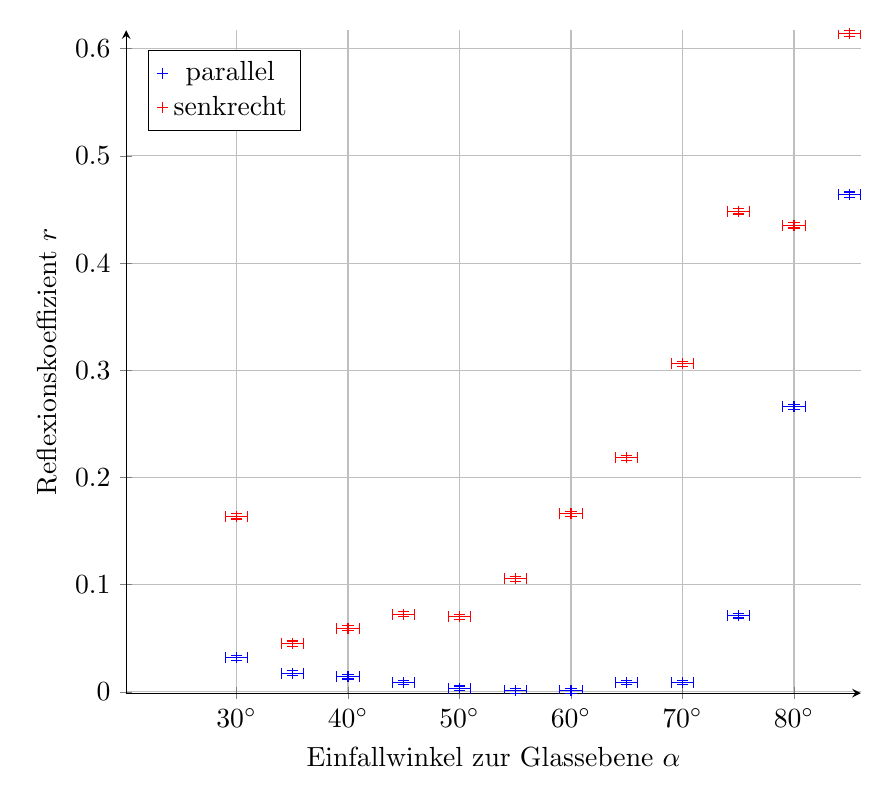
\begin{tikzpicture}
\begin{axis}[xticklabel=$\pgfmathprintnumber{\tick}^\circ$, width=.9\linewidth, height=10cm,
	axis y line=left, axis x line = bottom, xmin = 20.1, legend pos = north west,
	xmajorgrids = true,ymajorgrids = true,
	xlabel = {Einfallwinkel zur Glassebene $ \alpha $},
	ylabel = {Reflexionskoeffizient $ r $}]
	\addplot+ [only marks, mark=+, 
		error bars/.cd, x dir = both, x explicit,
		y dir = both, y explicit] 
	table[x=x,y=y, x error=xerr, y error=yerr] {
x	xerr	y	yerr
30	1	0.0317286652	0.002189285
35	1	0.0175054705	0.0021885191
40	1	0.0142231947	0.0021884051
45	1	0.0087527352	0.0021882676
50	1	0.0032822757	0.0021881956
55	1	0.0010940919	0.0021881851
60	1	0.0010940919	0.0021881851
65	1	0.0087527352	0.0021882676
70	1	0.0087527352	0.0021882676
75	1	0.0711159737	0.0021937102
80	1	0.2658643326	0.0022641981
85	1	0.4638949672	0.0024121673
	};
\addplot+ [only marks, mark=+, 
			error bars/.cd, x dir = both, x explicit,
			y dir = both, y explicit] 
		table[x=x,y=y, x error=xerr, y error=yerr] {
	x	xerr	y	yerr
	30	1	0.1637010676	0.002404058
	35	1	0.0450771056	0.0023748884
	40	1	0.059311981	0.0023766487
	45	1	0.0723606168	0.0023786824
	50	1	0.0699881376	0.0023782827
	55	1	0.1055753262	0.0023856646
	60	1	0.1660735469	0.0024049737
	65	1	0.2182680902	0.0024283353
	70	1	0.3060498221	0.0024811035
	75	1	0.4483985765	0.0026000698
	80	1	0.4353499407	0.0025875577
	85	1	0.6144721234	0.0027845832
		};
%	\addplot+[domain= -45:140, no marks, samples=100] {2043*(cos(x- 44.9940891727))^2};
\legend{parallel, senkrecht}
\end{axis}

\end{tikzpicture}
\caption{Reflexion von polarisierten Licht}
\label{fig:refp}
\end{figure}
Für parallel polarisiertes Licht ist zwischen \SI{55(1)}{\degree} und \SI{60(1)}{\degree} minimal. Somit liegt der Brewster-Winkel im Bereich $ \alpha_B = \SI{57,5(35)}{\degree} $.
Aus \eqref{eq:brew} erhält man daraus den Brechungsindex des Glases, aus \eqref{eq:err:brew} die dazugehörige Unsicherheit. Wir erhalten $ n = \num{1,57(22)} $.

\subsection{Optische Aktivität von Zuckerlösungen}
Ziel dieses Versuches ist es die Zuckerkonzentration einer Lösung anhand der optischen Aktivität zu bestimmen. Dazu sind als Hilfsmittel vier Zuckerlösungen mit bekannter Konzentration gegeben in gleich langen, transparenten Gefäßen wie die unbekannte Zuckerlösung.
Dazu wird das Licht zunächst durch einen ersten Polarisator in einer Ebene linear polarisiert. Daraufhin fällt das Licht durch die Zuckerlösung und danach durch einen zweiten Polarisator. Diesen zweiten Polarisator dreht man so, dass die Menge des transmittierten Lichts minimal wird. In diesem Fall ist der Polarisator genau rechtwinklig zur Polarisationsebene. Somit lässt sich der Drehwinkel $ \alpha $ in der Lösung aus dem Winkel $ \alpha_{12} $ zwischen den Polarisatoren errechnen durch
\begin{equation}
	\alpha = \alpha_{12} - \SI{90}{\degree}
\end{equation}
Nach \eqref{eq:opt_akt} ist der Drehwinkel proportional zur Konzentration der Lösung bei konstanter Länge. Also lässt sich eine Ausgleichsgerade 
\begin{equation}
	\alpha(c) = k\cdot c \label{eq:zucker-fit}
\end{equation}
durch die Messwerte legen. Dabei ist $ k $ eine Proportionalitätskonstante. Aus dieser Geraden lassen sich die Drehwinkel beliebiger Konzentrationen bestimmen.\\
Bei der Durchführung haben wir den Winkel minimaler Intensität nicht mithilfe des Photosensors bestimmt. Da dieser für kleine Intensitäten nicht fein genug misst, haben wir stattdessen ein weißes Blatt Papier hinter den zweiten Polarisator gehalten und den Winkel gesucht, unter dem der Lichtpunkt verschwindet. Auf diese Methode lässt sich der Winkel genauer einstellen, als man ihn auf der Skala ablesen kann.\\
Unsere Messwerte sind in Abbildung \ref{fig:zucker} graphisch dargestellt. Für die Ausgleichsgerade haben wir mit \textit{Gnuplot} nach dem \textit{Least-Square-Fit} Verfahren unsere Messwerte gegen \eqref{eq:zucker-fit} gefittet. Wir erhielten daraus $ k = \num{1.08+-.05} $. Dabei ist $ \num{.025} $ der von \textit{Gnuplot} angegebene statistische Fehler. Dazu schätzen wir einen weiteren Fehler gleicher Größe aus der Unsicherheit der Messwerte ab.
\begin{figure}[H]
\centering
\begin{tikzpicture}
\begin{axis}[yticklabel=$\pgfmathprintnumber{\tick}^\circ$, width=.9\linewidth, height=10cm,
	legend pos = north west, xmajorgrids,
	ylabel = {Drehwinkel $ \alpha $},
	xlabel = {Zuckerkonzentration $ c $ [\si{g/100.cm^{3}}]}]
	\addplot+ [only marks, mark=+, 
		error bars/.cd,
		y dir = both, y fixed = 2] 
	table[x=x,y=y] {
x	y
0	2
5	6
10	10
20	22
40	43
	};
	\addplot+[domain= 0:45, no marks] {1.07764705830693*x};
	\addplot+[domain=0:45, no marks, green, dashed] {29};
\legend{Meswerte, $ \num{1.078 }c $, Drehwinkel von \textit{u}}
\end{axis}

\end{tikzpicture}
\caption{$ c $-$ \alpha $-Diagramm des untersuchten Zuckers}
\label{fig:zucker}
\end{figure}
Stellt man \eqref{eq:zucker-fit} um, erhält man \begin{equation}
	c = \frac{\alpha}{k}
\end{equation}
Damit, und dem Fehler aus \eqref{eq:err} erhalten wir für die Konzentration der unbekannten Lösung $ c = \SI{27,0(23)}{\gram\per 100.\centi\meter^{3}} $

%\begin{figure}[H]
%\centering
%\begin{tikzpicture}
\begin{axis}[xticklabel=$\pgfmathprintnumber{\tick}^\circ$, width=.9\linewidth, height=10cm,
	axis y line=left, axis x line = bottom, xmin = 20.1]
	\addplot+ [only marks, mark=+, 
		error bars/.cd, x dir = both, x fixed=1,
		y dir = both, y fixed = 2] 
	table[x=x,y=y, x error=xerr, y error=yerr] {
x	xerr	y	yerr
30	1	138	2
35	1	38	2
40	1	50	2
45	1	61	2
50	1	59	2
55	1	89	2
60	1	140	2
65	1	184	2
70	1	258	2
75	1	378	2
80	1	367	2
85	1	518	2
	};
%	\addplot+[domain= -45:140, no marks, samples=100] {2043*(cos(x- 44.9940891727))^2};
\legend{Meswerte, $ 2043\cos^2(x-\SI{45,0}{\degree}) $}
\end{axis}

\end{tikzpicture}
%\caption{Reflektion senkrecht [Platzhalter]}
%\label{fig:refs}
%\end{figure}
\subsection{Kalkspat}
Wird der Laser durch einen Kalkspatkristall geschickt ist sichtbar, dass der Strahl sich aufteilt. Wird der Polarisationsfilter auf $ \SI{29}{\degree} $ eingestellt ist nur der untere Strahl sichtbar, bei $ \SI{120}{\degree} $ ist nur der obere Strahl sichtbar. 

\newpage
\section{Diskussion} 
\subsection{Gesetz von Malus}
Das Gesetz von Malus passt sehr gut zur Darstellung der von uns gemessenen Daten. Mit nur einer Ausnahme berühren alle Messpunkte die nach dem Gesetz von Malus gefittete Kurve. 

\subsection{$ \lambda /2 $ -Platte}
Bei einer Einstellung von $ 45^\circ $ wurde, wie erwartet, eine Drehung der Polarisationsebene von $ 90^\circ $ gemessen.
Bei einer Veränderung von $ 45^\circ $ auf $ 30^\circ $ wurde eine Drehung der Polarisationsebene von $ 30^\circ $ beobachtet, dies war ebenfalls erwartet.

\subsection{p- und s-polarisiertes Licht}
Vom Trend entsprechen die Kurven den theoretisch Erwarteten. Im Fall des parallel-polarisierten Lichts ist der Tiefpunkt im Bereich des Brewster-Winkels sichtbar geworden und die Lichtintensität ist in diesem Bereich fast nicht messbar. Auch bei senkrecht polarisierten Licht sind mit steigenden Brechungswinkeln zunehmende Reflexionskoeffizienten sichtbar. Jedoch sind hier auch einige Ausreißer zu sehen. Insbesondere die gemessenen Intensitäten bei \SI{30}{\degree} und \SI{75}{\degree} fallen aus der Reihe. \\
Eine Erklärung für die Streuung der Messwerte kann auch die beschriebenen zwei reflektierten Punkte sein. Dass zwei Punkte zu sehen sind, ist wahrscheinlich eine Folge dessen, dass es an der Glasplatte zwei Reflexionsebenen gibt. Neben der vorderen Ebene beim Einfall reflektiert das Licht auch an der hinteren Glasebene beim Ausfallen. Durch die Brechung beim Einfallen kommt es dabei zum Parallelversatz und es sind zwei Lichtpunkte zu sehen. \\
Da nach den Snellius'schen Brechungsgesetzen der Lichtstrahl in die hintere Plattenebene steiler einfällt, kann das Licht hier zu großen Teilen reflektiert werden. Daher könnte dies eine Erklärung für den Ausreißer bei \SI{30}{\degree} sein. \\
Der Brechungsindex des Glases liegt in einem sinnvollen Bereich. Der Brechungsindex von verschiedenen Glasen liegt im Bereich \num{1,5} bis \num{2.0} \cite{wiki:brech}. Der von uns bestimmte Wert $ n = \num{1.57(22)} $ passt in diesen Bereich. Jedoch haben wir in vorherigen Versuchen bereits Methoden kennengelernt, um den Brechungsindex mit einfacheren Mitteln genauer zu bestimmen. Es hat sich im Versuch zwar gezeigt, dass es möglich ist einen Brechungsindex so zu Bestimmen, ich halte es aber nicht für sinnvoll die Methode anzuwenden, wenn das einzige Ziel ist, den Brechungsindex eines Materials zu bestimmen.

\subsection{Optische Aktivität von Zuckerlösungen}
Der in der Theorie angenommene lineare Zusammenhang zwischen Konzentration der Lösung und Drehwinkel konnte im Versuch gut gezeigt werden. Die von uns erhaltenen Messwerte lassen sich durch eine Ursprungsgrade gut darstellen. Die Unsicherheit der ermittelten Konzentration ist mit etwa \SI{10}{\percent} zwar relativ hoch, jedoch lassen sich im allgemeinen Winkel noch viel genauer bestimmen, als es uns im Versuch möglich war. \\
Ich kann mir für dieses Verfahren praktische Anwendung vorstellen. Die in diesem Versuch ermittelten werte lassen sich relativ schnell und einfach ermitteln. Dies wäre technisch sogar voll automatisch umsetzbar. Will man nun die Lösungskonzentration von optisch aktiven Stoffen bestimmen, ist der Vorteil dieser Methode, dass sie "von außen" angewendet werden kann. Die Probe bleibt in Menge und Qualität vollständig erhalten.

\subsection{Kalkspat}
Wie erwartet ist der obere Strahl s-polarisiert und der untere p-polarisiert. Dies könnte beispielweise in der optischen Datenübertragung technisch genutzt werden. In einem Lichtleiter wird ein Signal senkrecht und das andere Signal parallel polarisiert Übertragen. Beim Empfänger werden diese dann mit einem Kalkspat wieder getrennt und können unabhängig verarbeitet werden.